%% Copyright 2018 H.\ Rabus
%
% This work may be distributed and/or modified under the
% conditions of the LaTeX Project Public License, either version 1.3
% of this license or (at your option) any later version.
% The latest version of this license is in
%   http://www.latex-project.org/lppl.txt
% and version 1.3 or later is part of all distributions of LaTeX
% version 2005/12/01 or later.
%
% This work has the LPPL maintenance status `author-maintained'.
%
% This work consists of the file texbsp.tex
%

\documentclass[smallheadings]{scrartcl}

%%% GENERAL PACKAGES %%%%%%%%%%%%%%%%%%%%%%%%%%%%%%%%%%%%%%%%%%%%%%%%%%%%%%%%%%
% inputenc allows the usage of non-ascii characters in the LaTeX source code
\usepackage[utf8]{inputenc}
\usepackage{graphicx} 
\usepackage{subfigure}
\usepackage{float}
\usepackage{fancyhdr}
%\graphicspath{ {/u/hnatiuka/Praktikum/PPI/} }

% Turn on the style
\pagestyle{fancy}
% Clear the header and footer
\fancyhead{}
\fancyfoot{}
% Set the right side of the footer to be the page number
\fancyfoot[R]{\thepage}

% title of the document
\title{Bericht zu Serie 1}
% optional subtitle
%\subtitle{Draft from~\today}
% information about the author
\author{%
  Arsen Hnatiuk,\\%
  Max Huneshagen 
}
\date{\today} 


%%% LANGUAGE %%%%%%%%%%%%%%%%%%%%%%%%%%%%%%%%%%%%%%%%%%%%%%%%%%%%%%%%%%%%%%%%%%
% babel provides hyphenation patterns and translations of keywords like 'table
% of contents'
\usepackage[ngerman]{babel}

%%% HYPERLINKS %%%%%%%%%%%%%%%%%%%%%%%%%%%%%%%%%%%%%%%%%%%%%%%%%%%%%%%%%%%%%%%%
% automatic generation of hyperlinks for references and URIs
\usepackage{hyperref}

%%% MATH %%%%%%%%%%%%%%%%%%%%%%%%%%%%%%%%%%%%%%%%%%%%%%%%%%%%%%%%%%%%%%%%%%%%%%
% amsmath provides commands for type-setting mathematical formulas
\usepackage{amsmath}
% amssymb provides additional symbols
\usepackage{amssymb}
% HINT
% Use http://detexify.kirelabs.org/classify.html to find unknown symbols!

%%% COLORS %%%%%%%%%%%%%%%%%%%%%%%%%%%%%%%%%%%%%%%%%%%%%%%%%%%%%%%%%%%%%%%%%%%%
% define own colors and use colored text
\usepackage[pdftex,svgnames,hyperref]{xcolor}

%%% Code Listings %%%%%%%%%%%%%%%%
% provides commands for including code (python, latex, ...)
\usepackage{listings}
\definecolor{keywords}{RGB}{255,0,90}
\definecolor{comments}{RGB}{0,0,113}
\definecolor{red}{RGB}{160,0,0}
\definecolor{green}{RGB}{0,150,0}
\lstset{language=Python, 
        basicstyle=\ttfamily\small, 
        keywordstyle=\color{keywords},
        commentstyle=\color{comments},
        stringstyle=\color{red},
        showstringspaces=false,
        identifierstyle=\color{green},
        }


\usepackage{paralist}
\usepackage{nicefrac}

\renewcommand{\texttt}[1]{%
  \begingroup
  \ttfamily
  \begingroup\lccode`~=`/\lowercase{\endgroup\def~}{/\discretionary{}{}{}}%
  \begingroup\lccode`~=`[\lowercase{\endgroup\def~}{[\discretionary{}{}{}}%
  \begingroup\lccode`~=`.\lowercase{\endgroup\def~}{.\discretionary{}{}{}}%
  \catcode`/=\active\catcode`[=\active\catcode`.=\active
  \scantokens{#1\noexpand}%
  \endgroup
}
\newcommand*\justify{%
  \fontdimen2\font=0.4em% interword space
  \fontdimen3\font=0.2em% interword stretch
  \fontdimen4\font=0.1em% interword shrink
  \fontdimen7\font=0.1em% extra space
  \hyphenchar\font=`\-% allowing hyphenation
}
% setting the font style for input und returns in description items
\newcommand{\initem}[2]{\item[\hspace{0.5em} {\normalfont\ttfamily{#1}} {\normalfont\itshape{(#2)}}]}
\newcommand{\outitem}[1]{\item[\hspace{0.5em} \normalfont\itshape{(#1)}]}
\newcommand{\bfpara}[1]{
	
	\noindent \textbf{#1:}\,}

\begin{document}

% generating the title page
\maketitle
% generating the table of contents (requires to run pdflatex twice!)
\tableofcontents
\bigskip

\hrule
\hrule

%%% BEGIN OF CONTENT %%%%%%%%%%%%%%%%%%%%%%%%%%%%%%%%%%%%%%%%%%%%%%%%%%%%%%%%%%

\section{Einleitung}
Aus der Theorie der Taylorentwicklung kann man ein günstiges Verfahren zur Approximation der ersten und zweiten Ableitungen einer Funktion ableiten: 
\begin{align}
\label{eq:1_abl}
f'(x)=\underbrace{\frac{f(x+h)-f(x)}{h}}_{:=D_h^{(1)}(x)}+\mathcal{O}(h)
\end{align}
bzw.
\begin{align}
\label{eq:2_abl}
f''(x)=\underbrace{\frac{f(x+h)-2f(x)+f(x-h)}{h^2}}_{:=D_h^{(2)}(x)}+\mathcal{O}(h^2)
\end{align}
mit der Differenziationsschrittweite $h$.

Dieses Verfahren kann sehr nützlich in der numerischen Mathematik sein, jedoch hängt seine Genauigkeit, wie bei jedem Approximationsverfahren, stark von dem Wert der eingegebenen Parameter ab. Deswegen wird eine Studie der Genauigkeit für die sinnvolle Nutzung des Verfahrens benötigt. Die im Teil 1 erstellte Klasse \texttt{Differenzieren} in \texttt{differnzieren.py} erlauben eine numerische Analyse der Beziehung zwischen der Genauigkeit der Approximation und den Parametern. 

\section{Theorie}
Die in der Einleitung genannten Formeln  \eqref{eq:1_abl} und~\eqref{eq:2_abl}  lassen sich aus der Theorie der Taylorentwicklung wie folgt ableiten:
für eine glatte reellwertige Funktion $f$, für $x\in\mathbb{R}$ und für $h$ in einer passenden Umgebung von $x$ gilt:
\begin{align}
f(x+h)&=\sum_{k=0}^{\infty}\frac{f^{(k)}(x)}{k!}h^k\\
&=f(x)+f'(x)h+\sum_{k=2}^{\infty}\frac{f^{(k)}(x)}{k!}h^k.
\label{eq:taylor_neg_h}
\end{align}
Das Lösen nach $f'(x)$ liefert:
\begin{align}
f'(x)&=\frac{f(x+h)-f(x)}{h}-\sum_{k=2}^{\infty}\frac{f^{(k)}(x)}{k!}h^{k-1}\\
&=\frac{f(x+h)-f(x)}{h}+\mathcal{O}(h).
\end{align}
Die zweite Formel erhält man auf eine ähnliche Weise. Wir können die Taylorentwicklung auf ein negatives $h$ anwenden:
\begin{align}
f(x-h)&=\sum_{k=0}^{\infty}\frac{f^{(k)}(x)}{k!}(-h)^k\\
&=f(x)-f'(x)h+\frac{f''(x)h^2}{2} +\sum_{k=3}^{\infty}\frac{f^{(k)}(x)}{k!}(-h)^k.
\label{eq:taylor_pos_h}
\end{align}
Addition von \eqref{eq:taylor_pos_h} und \eqref{eq:taylor_neg_h} liefert:
\begin{align}
f(x+h)+f(x-h)=2f(x)+f''(x)h^2+\sum_{k=2}^{\infty}\frac{f^{(2k)}(x)}{(2k)!}h^{2k}.
\end{align}
Das Lösen nach $f''(x)$ ergibt:
\begin{align}
f''(x)=\frac{f(x+h)+f(x-h)-2f(x)}{h^2}+\mathcal{O}(h^2).
\end{align}


Ein anderer wichtiger Begriff für die Bearbeitung folgender Experimente ist die Periodizität der Sinus Abbildung und seiner Ableitungen. Zu einem gegebenen $j\in\mathbb{R}$ ist die Periode von $\sin(jx)$ gleich $\frac{2\pi}{j}$. Die Ableitungen von $\sin(jx)$ verhalten sich auf die gleiche Weise.

\section{Experimente}

\paragraph{Experiment 1}
Für die Veranschaulichung der Genauigkeit der Approximation von den Ableitungen bei Schrittweiten $\frac{\pi}{3}$, $\frac{\pi}{4}$, $\frac{\pi}{5}$ und $\frac{\pi}{10}$ wurde ein Programm geschrieben (\texttt{hauptprogramm2.py}), das den Sinus und seine ersten beiden Ableitungen (approximiert und exakt) im Intervall $\left[a,b\right]:=\left[0,\pi\right]$ plottet. Das Ergebnis ist in Abbildung~\ref{im:ablplot} dargestellt.

\paragraph{Experiment 2}
Im zweiten Experiment soll der maximale Fehler der Approximation 
\begin{align}
e_h^{(k)}:=\max\limits_{i=0,\dots,p}\vert f^{(k)}(x_i)-D_h^{(k)}x_i\vert\text{,~~~~~~~~}k=1,2
\end{align}
wiederum für $f(x)=\sin(x)$ in Abhängigkeit der Differenziationsschrittweite $h$ betrachtet werden. Besonderer Fokus soll hierbei auf das Konvergenzverhalten von $e_h^{(k)}$ gelegt werden. Aus \eqref{eq:1_abl} und \eqref{eq:2_abl} ist sofort ersichtlich, dass aus mathematisch naiver Sicht $e_h^{(k)}\sim h^k$ zu erwarten sein wird. 

\paragraph{Experiment 3}
Weiterhin wird das Konvergenzverhalten von $e_h^{(k)}$ für die Funktion $f_j(x)=\sin(jx)$ untersucht und mit dem des Sinus verglichen. In Experiment~3 wird zunächst der Fall $j<1$ betrachtet. Nach der Bemerkung zur Periodizität von $f_j$ in Abschnitt~\ref{sec:Theo} entspricht dies einer Streckung des Sinus entlang der Abszisse.

\paragraph{Experiment 4}
Im letzten Experiment wird analog zu Experiment~3 vorgegangen, allerdings wird nun der Fall $j>1$ untersucht, also der entlang der x-Achse gestauchte Sinus.


\section{Analyse der Experimente}

\paragraph{Experiment 1}

\begin{figure}[H]
	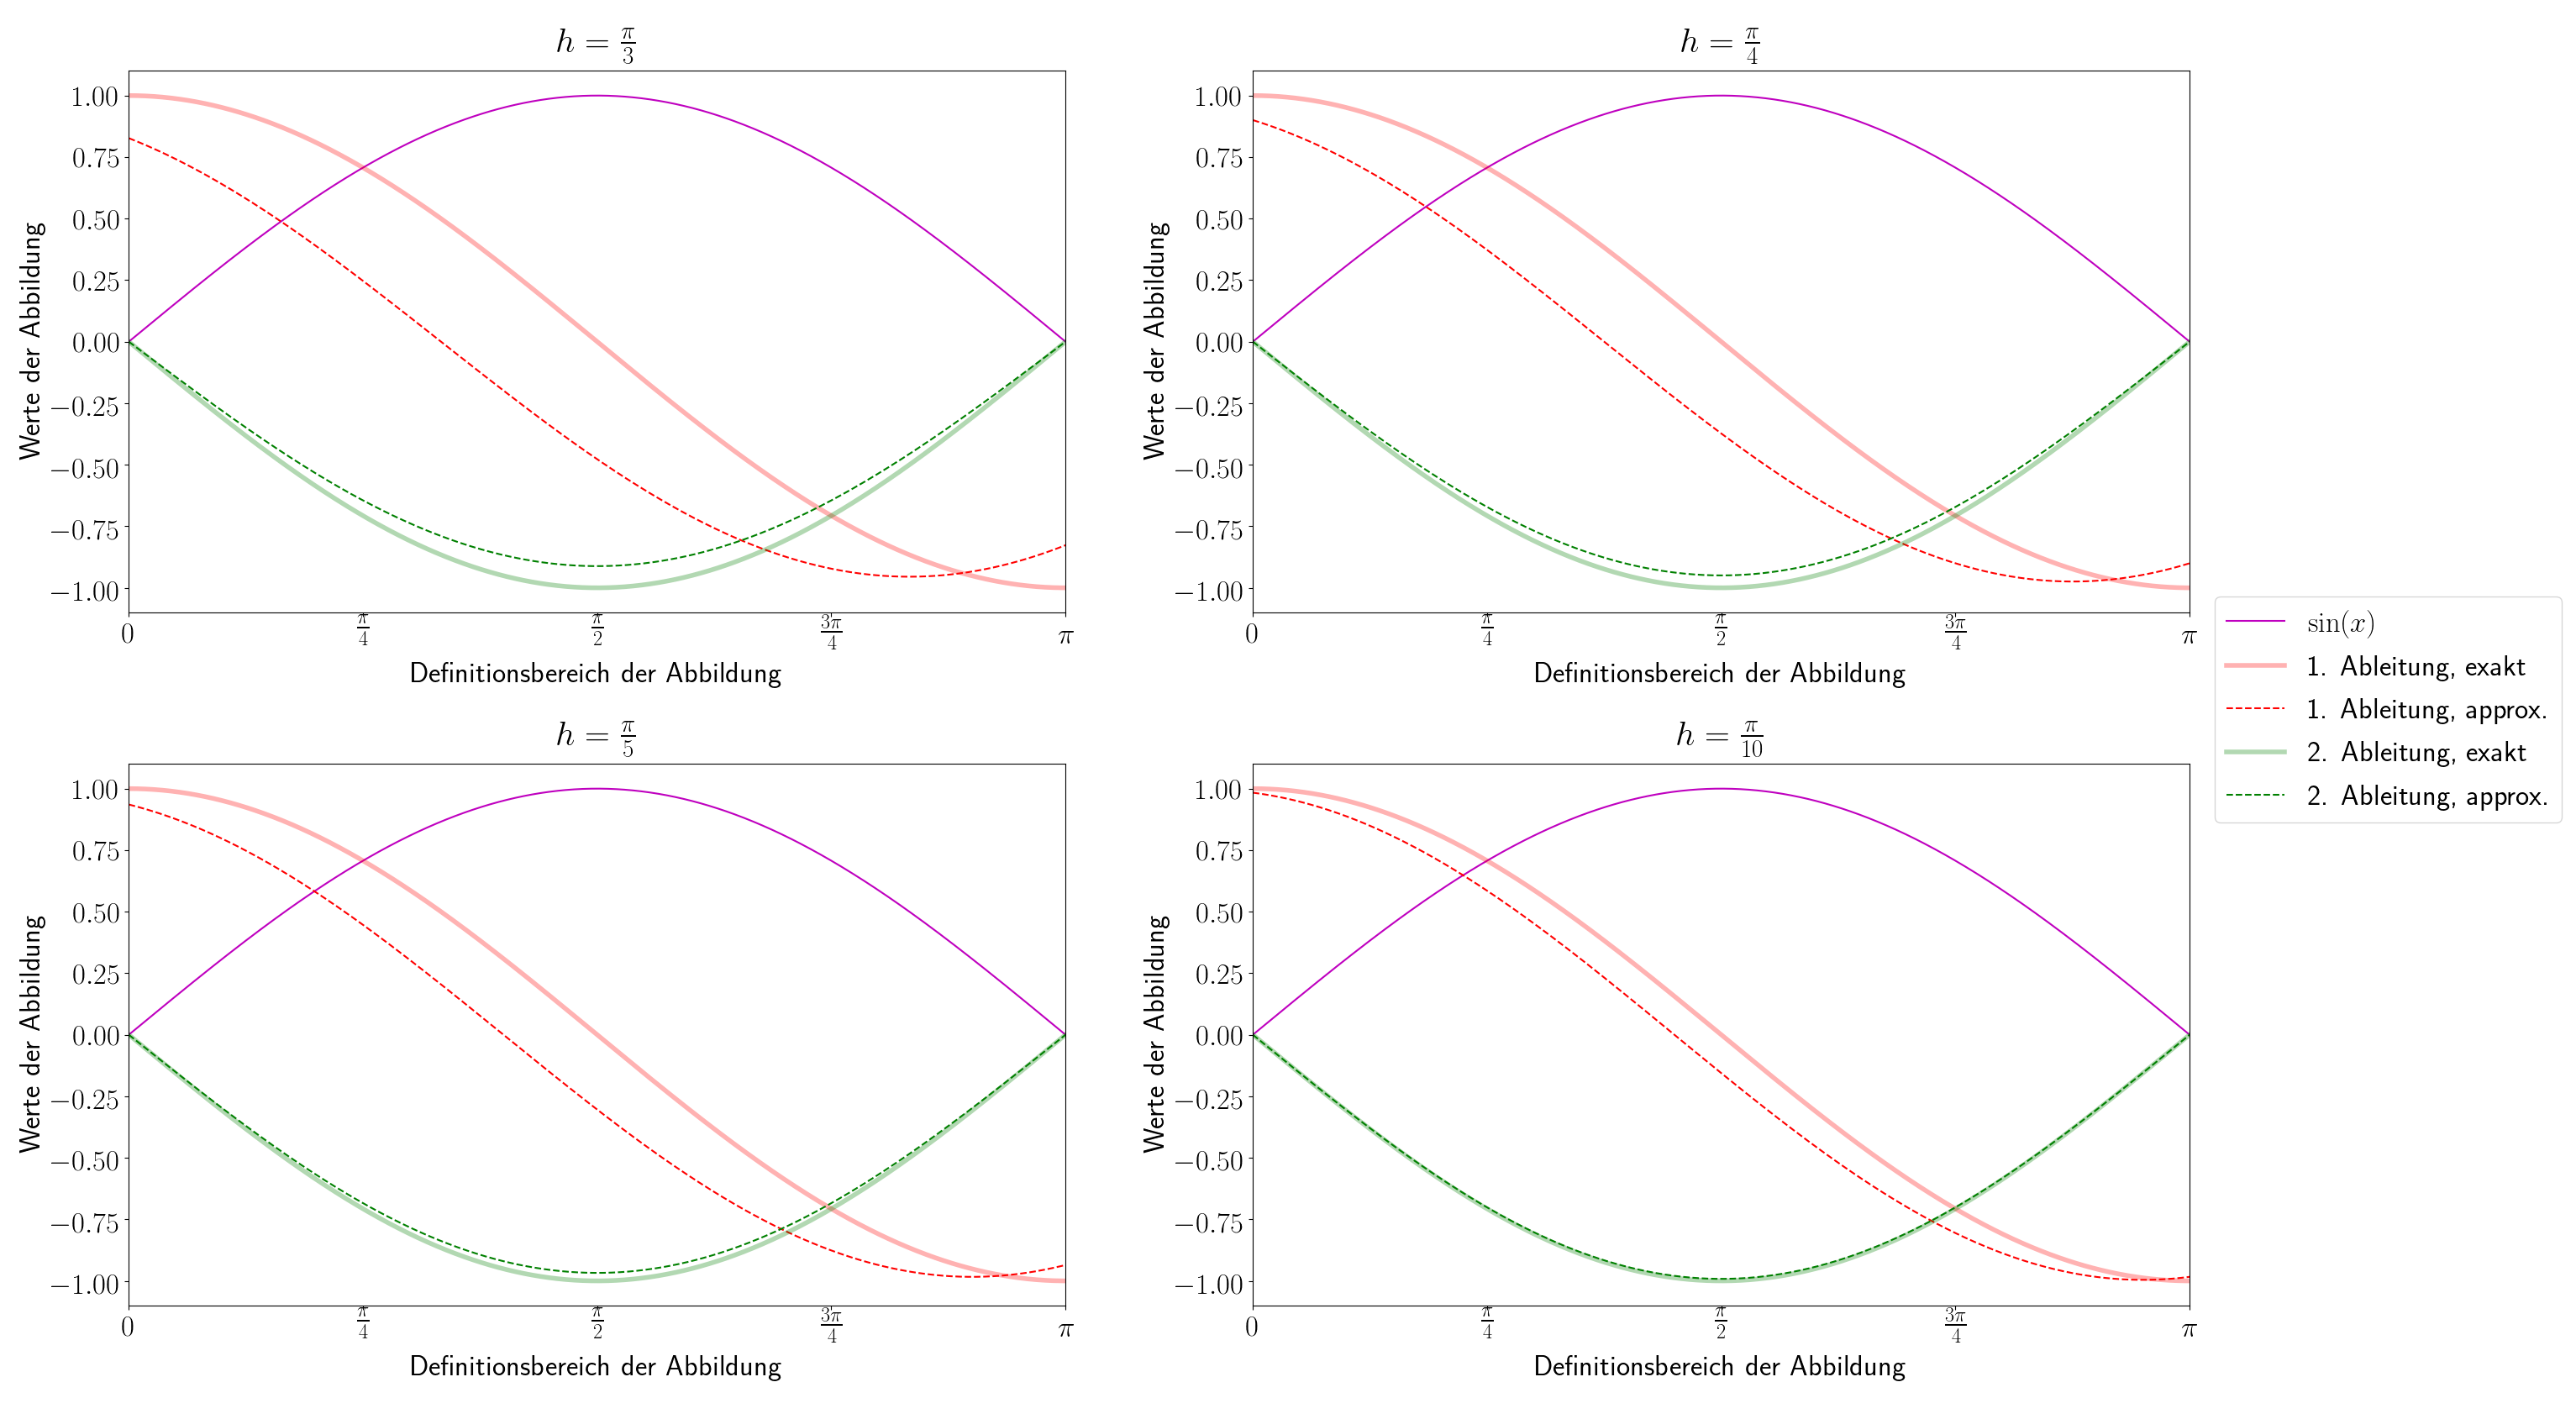
\includegraphics[width=\linewidth]{Bilder/fkt_abb.png}
	\caption{Die approximierten Ableitungen für verschiedene Schrittweiten (Experiment 1).}
	\label{im:ablplot}
\end{figure}

Aus der graphischen Ausgabe des ersten Experiments in Abb.~\ref{im:ablplot} wird dreierlei ersichtlich; zum Ersten wird die Approximation der beiden Ableitungen mit sinkendem $h$ genauer. Dies stimmt mit der Theorie überein, weil wir erwarten, dass der Fehler in der ersten bzw. zweiten Ableitung der Ordnung $\mathcal{O}(h)$ bzw. $\mathcal{O}(h^2)$ ist. 

Zweitens ist die die Approximation der ersten Ableitung im Vergleich zu den genauen Daten nach Rechts verschoben. Dies ist auch erwartet, der Grund dafür liegt in der Approximationsformel für die erste Ableitung \ref{eq:1_abl}. Man sieht dort, dass die approximierte Tangente nicht um den Punkt $x$ zentriert ist, sondern um den Mittelpunkt zwischen $x+h$ und $x$. Folglich ist die Approximation um $\frac{h}{2}$ nach rechts verschoben. Dies passiert nicht bei der zweiten Ableitung, weil die entsprechende Formel \ref{eq:2_abl} sowohl auf $x+h$, als auch auf $x-h$ beruht. Dieser Effekt wurde bereits in der Schnittstellendokumentation der Funktion \texttt{Differenzieren.ablapprox} besprochen.

Schließlich ist die Approximation der zweiten Ableitung für diese Schrittweiten genauer als die erste. Wie die erste Beobachtung, liegt dies an die Ordnung der entsprechenden Fehler nach \eqref{eq:1_abl} bzw.~\eqref{eq:2_abl}. Für $h=\frac{\pi}{4}$, $\frac{\pi}{5}$ und $\frac{\pi}{10}$ ist $h^2<h$, und folglich soll die Approximation der zweiten Ableitung genauer sein, als die erste. Für $h=\frac{\pi}{3}$ lässt sie die höhere Genauigkeit der zweiten Ableitung durch die oben beschriebene Verschiebung in der ersten Ableitung erklären. 

\paragraph{Experiment 2}
%hier Referenz zu Abbildung 2 zu schreiben


Der Fehlerplot zeigt drei verschiedene Tendenzen im Fehlerverhalten in Abhängigkeit von der Schrittweite $h$. In dem mittleren Bereich der Schrittweite (ungefähr für $h\in\left[10^{-8}, 1\right]$ für die erste Ableitung und $h\in[10^{-3}, 1] $ für die zweite) verhält sich der Fehler genau so, wie es die Approximationsformeln andeuten; er ist linear zu $h$ im Fall der Approximation der ersten Ableitung und quadratisch in $h$ im Fall der Approximation der zweiten Ableitung. 

\begin{figure}[H]
	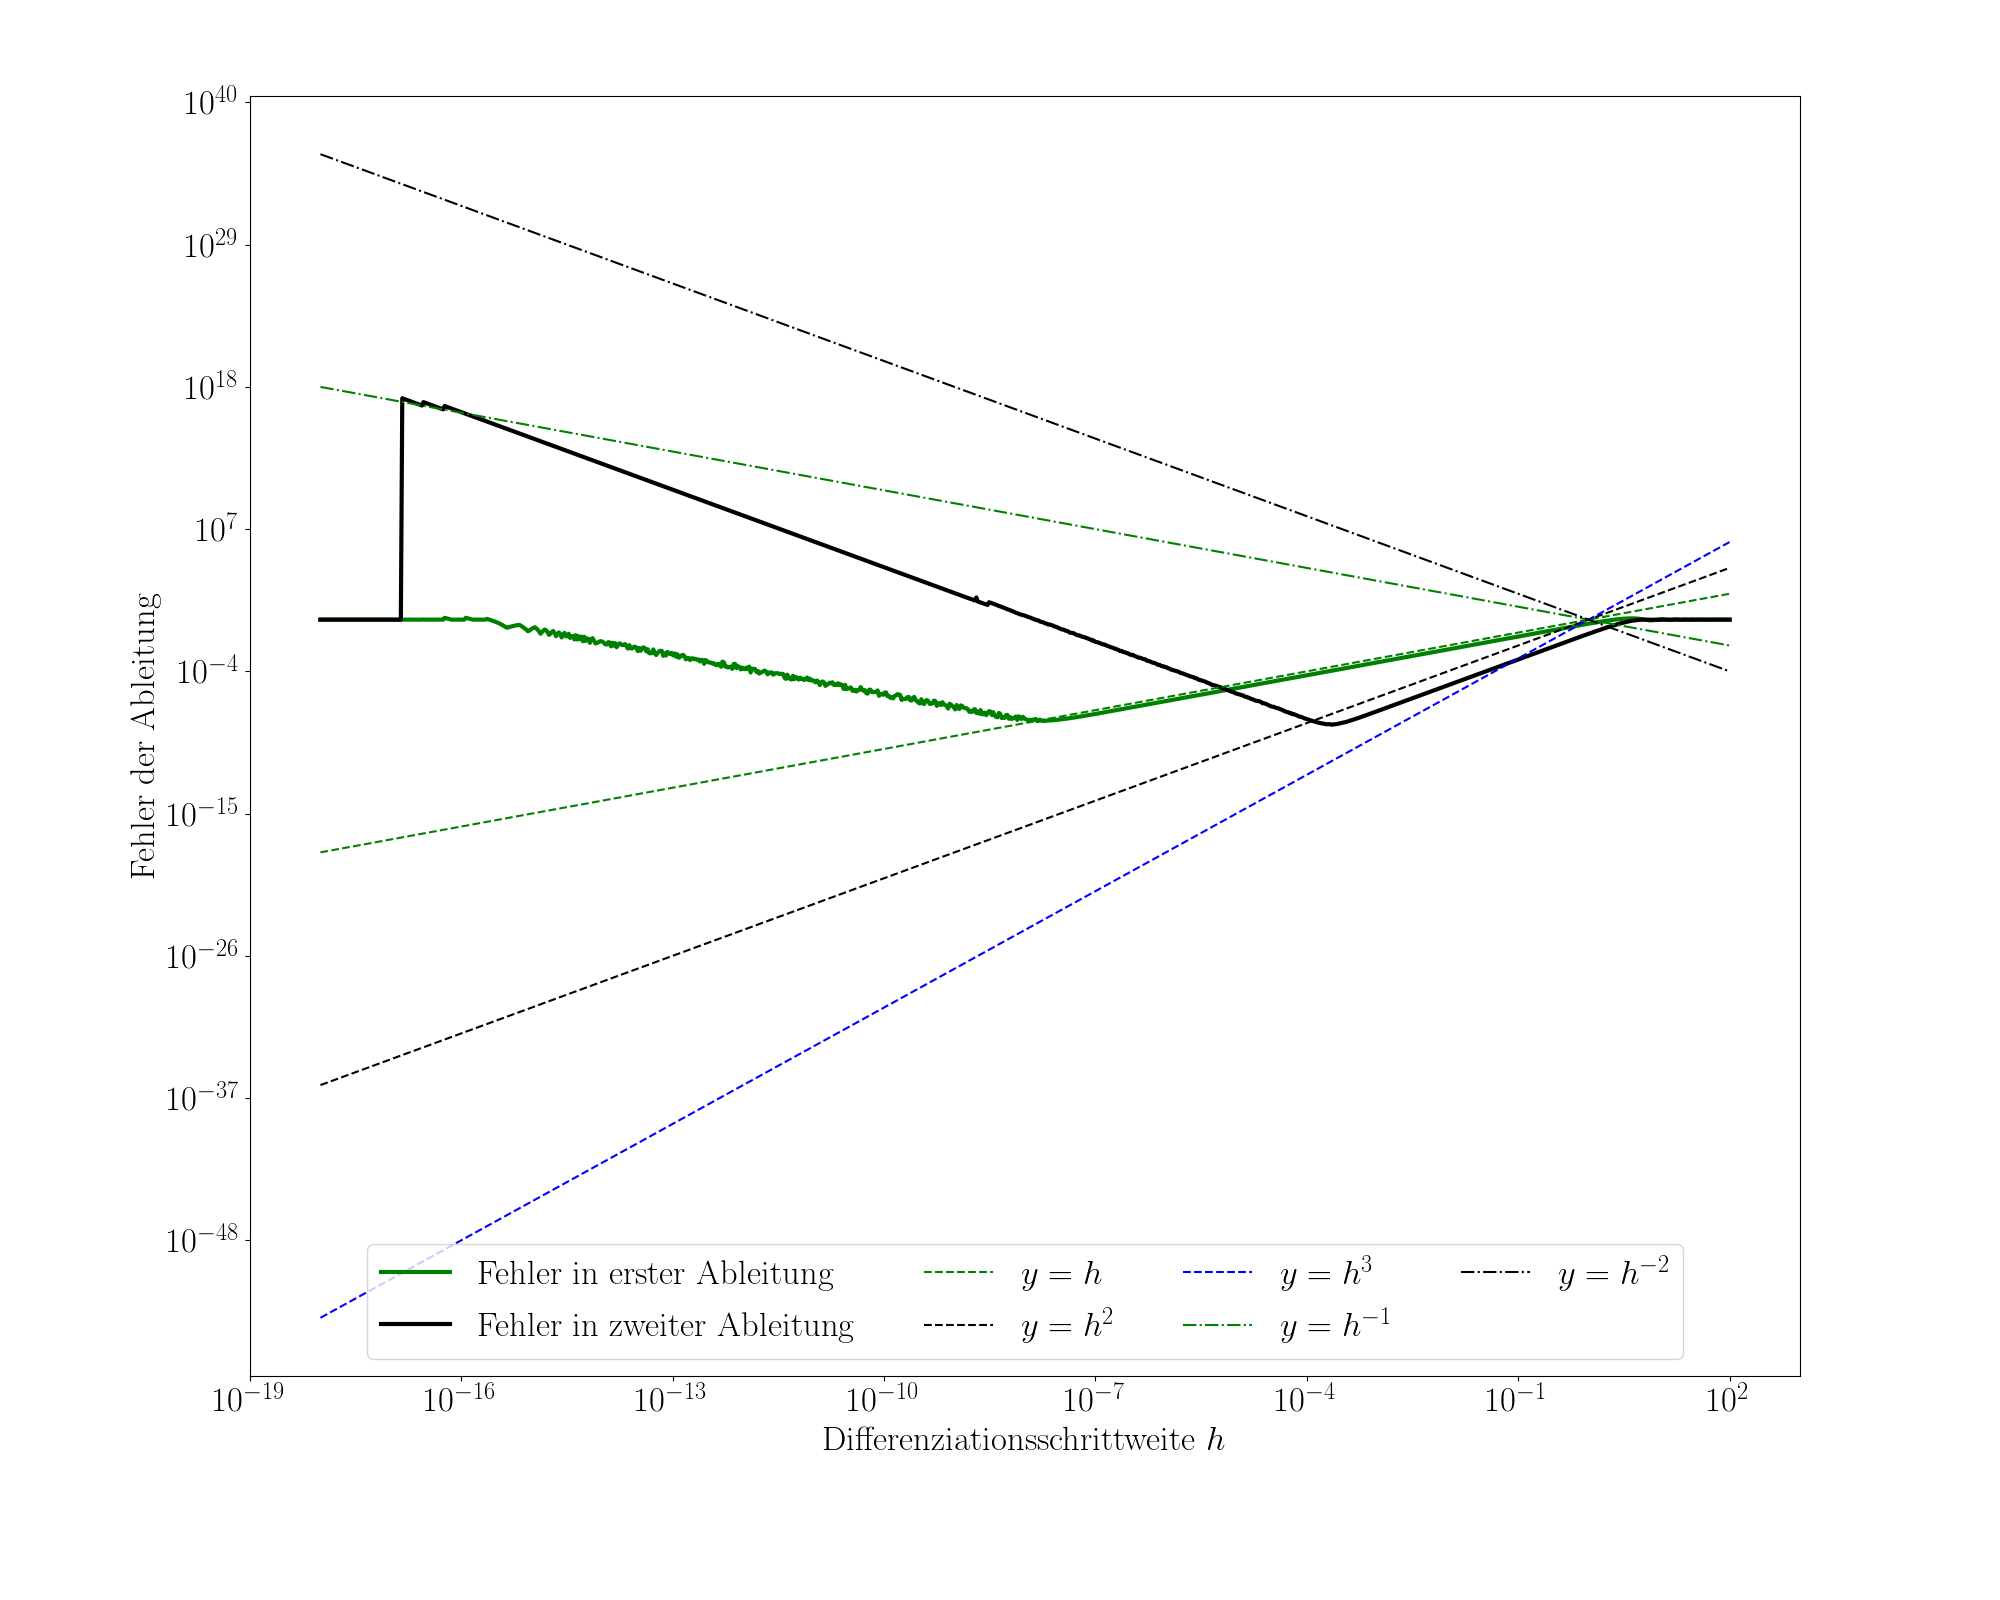
\includegraphics[width=\linewidth]{Bilder/errplot_lang}
	\caption{Maximaler Fehler der beiden ersten Ableitungen des Sinus im Abhängigkeit der Differenziationsschrittweite $h$.}
	\label{im:ablplot}
\end{figure}

Dieses Verhalten ändert sich bei Schrittweiten, die größer als 1 sind. In diesem Bereich konvergiert der Fehler für beide Approximationen gegen 1 für $h\gg1$. Der Grund dafür lässt sich auch aus den Formeln ablesen. Für $f(x)=\sin(x)$ gilt, dass der Zähler des Differenzenquotienten $f(x+h)-f(x)$ betragsmäßig niemals größer als 2 ist. Analog ist der Betrag von $f(x+h)-2f(x)+f(x-h)$ durch 4 beschränkt. Folglich geht bei $h\rightarrow\infty$ der gemäß \eqref{eq:1_abl} bzw.~\eqref{eq:2_abl} approximierte Wert der beiden Ableitungen für alle Punkte $x$ gegen 0. Da diese Werte mit denen der Kosinus bzw. negativen Sinus Abbildungen verglichen werden (diese erreichen im Intervall $\left[0,\pi\right]$ stets den Wert $1$ oder $-1$), konvergiert der maximale Fehler gegen 1. 

Ein anderes Verhalten des Fehlers beobachtet man für sehr kleine Schrittweiten (kleiner als $10^{-8}$ für die erste und $10^{-3}$ für die zweite Ableitung).
In den genannten Bereichen gilt in etwa:
\begin{align}
e_h^{(k)}\sim h^{-k}.
\end{align}
Der Grund hierfür liegt in der finiten Genauigkeit der \texttt{numpy.sin}-Funktion. Während arithmetischer Operationen werden nur 16 Stellen Genauigkeit benutzt (\texttt{\justify numpy.sin(1)-numpy.sin(1+10**-17)}  liefert \texttt{0}). Folglich unterscheiden sich \texttt{\justify numpy.sin(x+h)} und \texttt{numpy.sin(x)} für kleine $h$ in einer Umgebung von $\frac{\pi}{2}$ nur um die allerletzten Nachkommastellen. Also tritt im Ausdruck \texttt{numpy.sin(x+h)-numpy.sin(x)} für genügend kleine Werte von $h$ ein \glqq Rauschen\grqq auf, der Nenner von \eqref{eq:1_abl} bzw.~\eqref{eq:2_abl} wird auch in den vorderen Stellen eine statistisch verteilte Größe. Das gleiche gilt auch für \texttt{\justify numpy.sin(x-h)+numpy.sin(x+h)-2*numpy.sin(h)}. Die approximierte $k$-te Ableitung skaliert nun also mit dem Nenner des Differenzenquotienten: $e_h^{(k)}\sim h^{-k}$. Dieser Verlauf ist in Abb.~\ref{im:ablplot}
sichtbar, ebenso wie das rauschen um etwa eine Zehnerpotenz (i.~e.~Rauschen in der ersten Stelle.

Das besagte Rauschen verschwindet wieder für $h\leq 10^{-16}$. Stattdessen liefert $e_h^{(k)}$ den Wert 1 für die erste und zweite Ableitung. 
Für beide Ableitungen ist der Fehler in diesem Fall 1. Dies liegt daran, dass \texttt{numpy.sin(x)=numpy.sin(x + 10**-16)}, also sind die approximierten Werte immer 0. Wie im Fall der großen $h$ ist der Fehler dann immer 1.

\begin{figure}[H]
	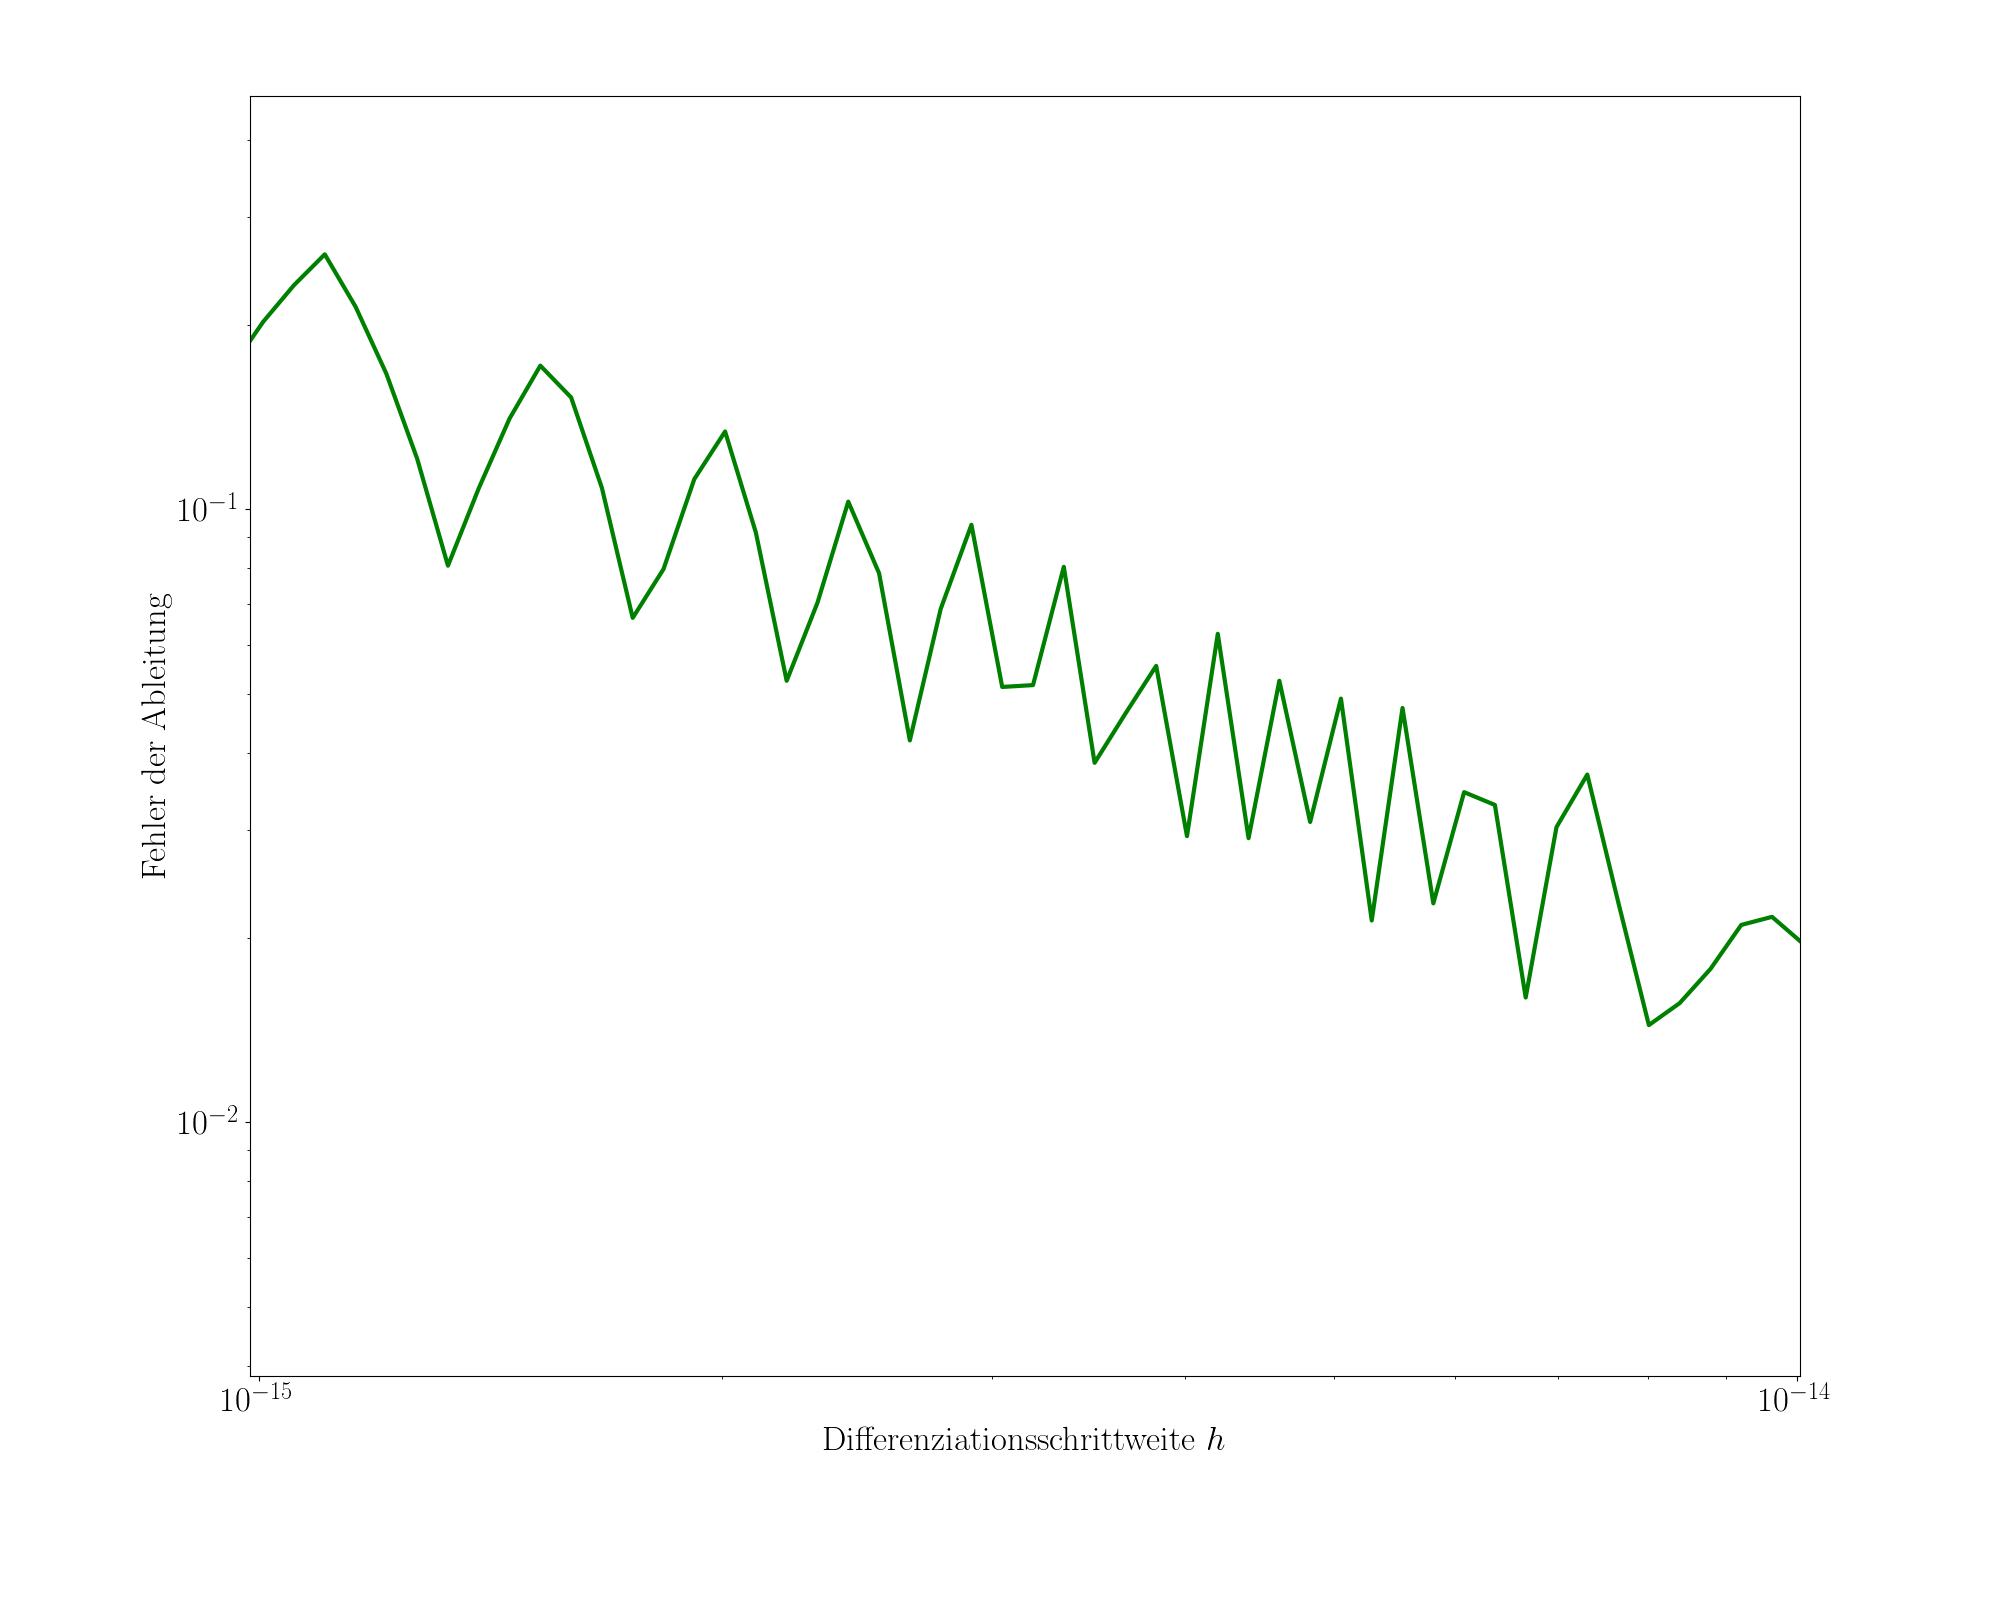
\includegraphics[width=\linewidth]{Bilder/rauschen}
	\caption{Vergrößerte Darstellung des Rauschens in der ersten Ableitung}
	\label{im:rauschen}
\end{figure}

\paragraph{Experiment 3}

Für $j\in\left(0,1\right]$ sinkt der absolute Wert von $e_h^{(k)}$ im Vergleich zum oben diskutierten Fall $j=1$ für alle $h$ im Bereich der erwarteten Konvergenz (s.\,Experiment 2). Das Absinken des Wertes für $e_h^{(k)}$ für kleine $j$ ist damit erklärbar, dass $j\rightarrow 0$ einer Vergrößerung der Periode des Sinus entspicht, die analog zu einer Verringerung von $h$ sein muss. Da $e_h^{(k)}$ in diesen Bereichen monoton steigend in $h$ ist, führt dies zu einer Verringerung des Fehlers (s.\,Abb~\ref{im:errplot_j_0004}~und~\ref{im:errplot_j_0100}). Weiterhin lässt sich beobachten, dass sich der Wert von $h_{krit}^{(k)}$, an dem sich das Konvergenzverhalten vom vorhergesagten zu $h^{-k}$ ändert, mit $j\rightarrow 0$ steigt. Dies rührt daher, dass die Funktion für kleine $j$ flacher wird (da ein $j^k$ als innere Ableitung auftritt) und somit die oben behandelte Auslöschung im Zähler von $e_h^{(k)}$ bereits bei größeren $h$ auftreten kann. Auch die Konvergenz $e_h^{(k)}\rightarrow 1$ für $h\rightarrow \infty$ ist für kleine $j$ nicht mehr gegeben, vielmehr konvergieren die Fehler gegen $j^k$, da der Betrag der ersten Ableitung hierdurch beschränkt ist und $e_h^{(k)}\rightarrow 0$ für $h\rightarrow \infty$ wie oben besprochen. Ebenso tritt letztgenannte Konvergenz für kleine $j$ später ein, für $j<0.05$ ist sie im geplotteten Bereich $\left[10^{-17},10^{2}\right]$ nicht mehr zu beobachten. Die Bereiche der verschiedenen Proportionalitäten aus Experiment~2 bleiben also für kleinere $j$ erhalten, ändern aber ihre Lage.

\paragraph{Experiment 4}

Für $j>1$ ist gewissermaßen der umgekehrte Effekt im Vergleich zu Experiment~3 zu erkennen (s.\,Abb.~\ref{im:errplot_j_0400},\ref{im:errplot_j_5000} sowie \ref{im:errplot_j_10000}); der Wert des Fehlers steigt im Bereich des erwarteten Verhaltens  mit $j$, der Bereich, ab dem das Rauschen beginnt, verschiebt sich dafür hin zu kleineren $h$. Die Konvergenz $e_h^{(k)}\rightarrow j^k$ tritt für große $j$ schon deutlich eher auf. Da $j^2>j$ für $j>1$ ist in diesem Bereich der Fehler der ersten Ableitung anders als im Fall von Experiment~3 kleiner als der der zweiten. Zur Erklärung dieser Effekte lässt sich ganz analog zu Experiment~3 argumentieren; die Erhöhung von $j$ entspricht einer Erhöhung der Frequenz des Sinus (bzw.~einer Verringerung der Periode), was zum gleichen qualitativen Ergebnis führen muss wie eine Vergrößerung von $h$ und damit zum  gegenteiligen Verhalten zu Experiment~3. Des Weiteren tritt die Tendenz $e_h^{(k)}\rightarrow 0$ für $h\rightarrow 0$ im betrachteten Breich nicht auf für $j<4$, da die Werte der $k$-ten Ableitung um $j^k$ größer werden als im Fall $j=1$ und somit der Nenner von $e_h^{(k)}$ erst für kleinere $h$ aufgrund der endlichen Rechengenauigkeit $0$ ergibt wie in der Auswertung von Experiment 2 beschrieben.


\begin{figure}[H]
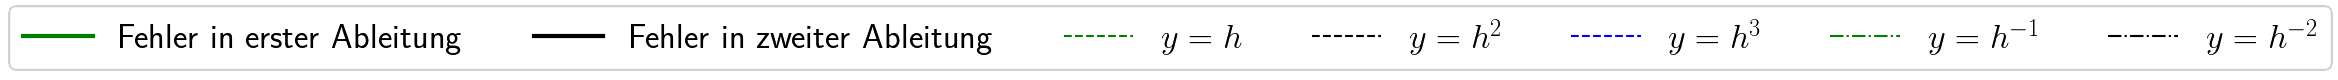
\includegraphics[width=\textwidth]{Bilder/legende}
\subfigure[$j=1$]{\label{im:errplot_j_0100}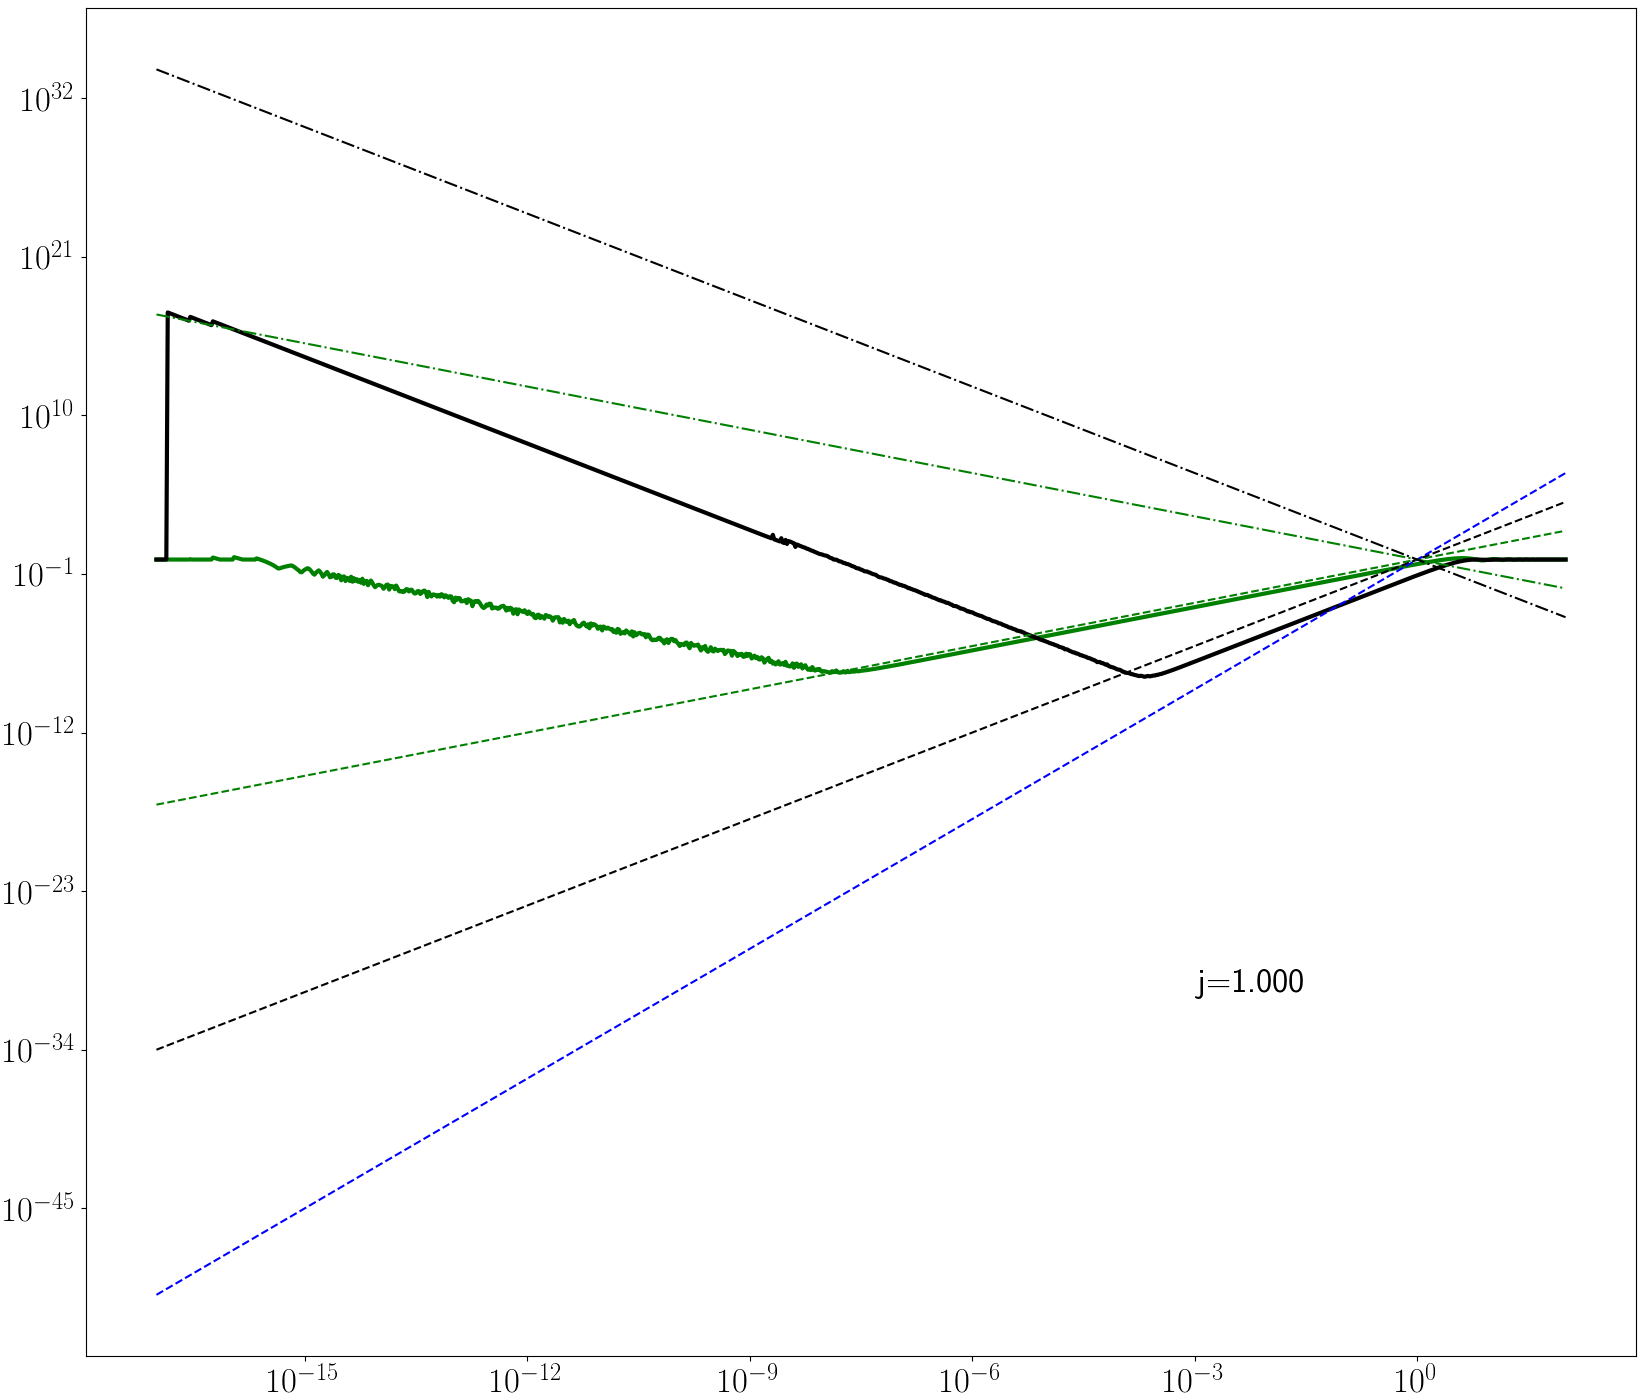
\includegraphics[width=.5\textwidth]{Bilder/errplot_j_0100.png}}
\subfigure[$j=0.04$]{\label{im:errplot_j_0004}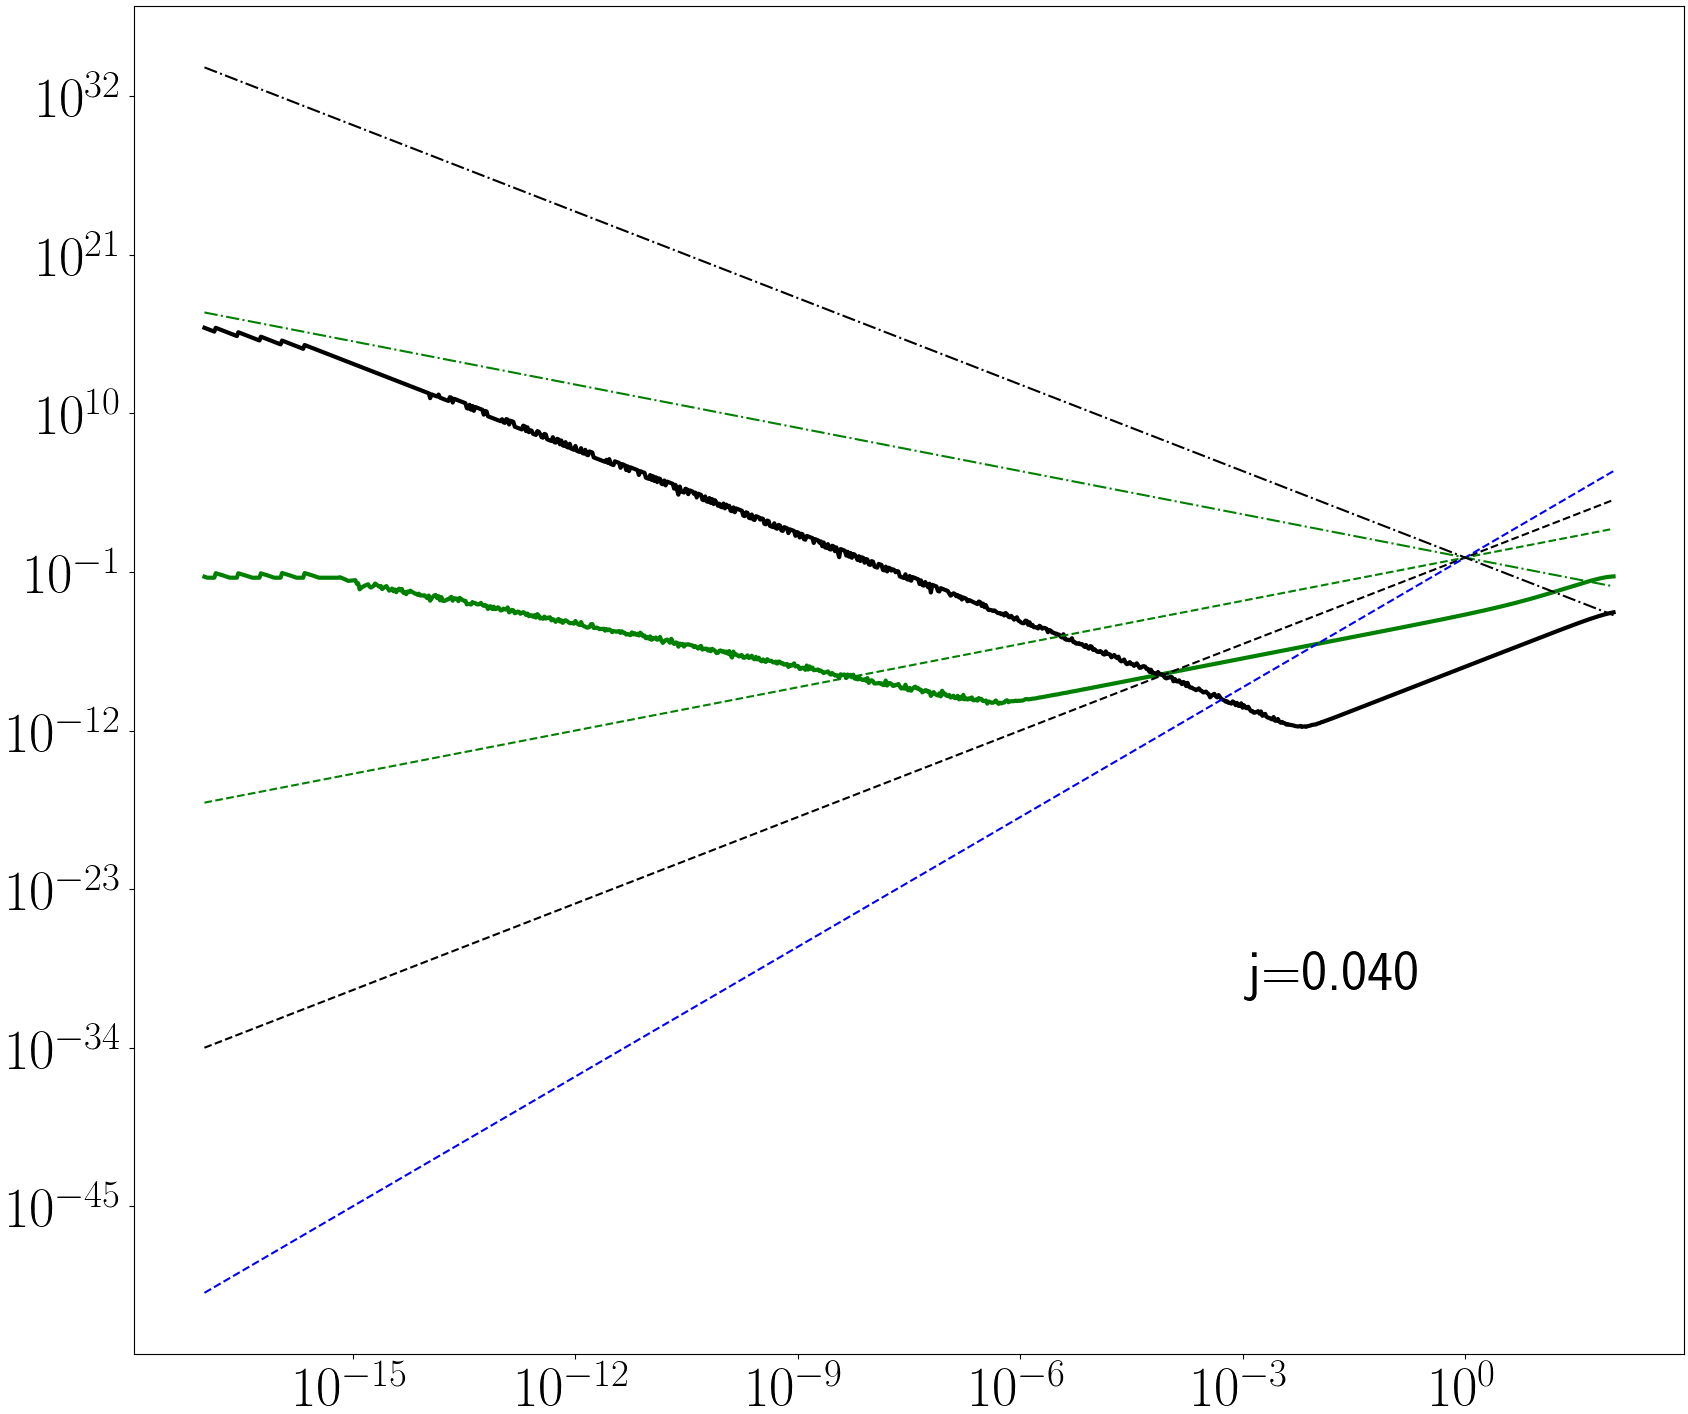
\includegraphics[width=.5\textwidth]{Bilder/errplot_0004.png}}
\subfigure[$j=0.5$]{\label{im:errplot_j_0050}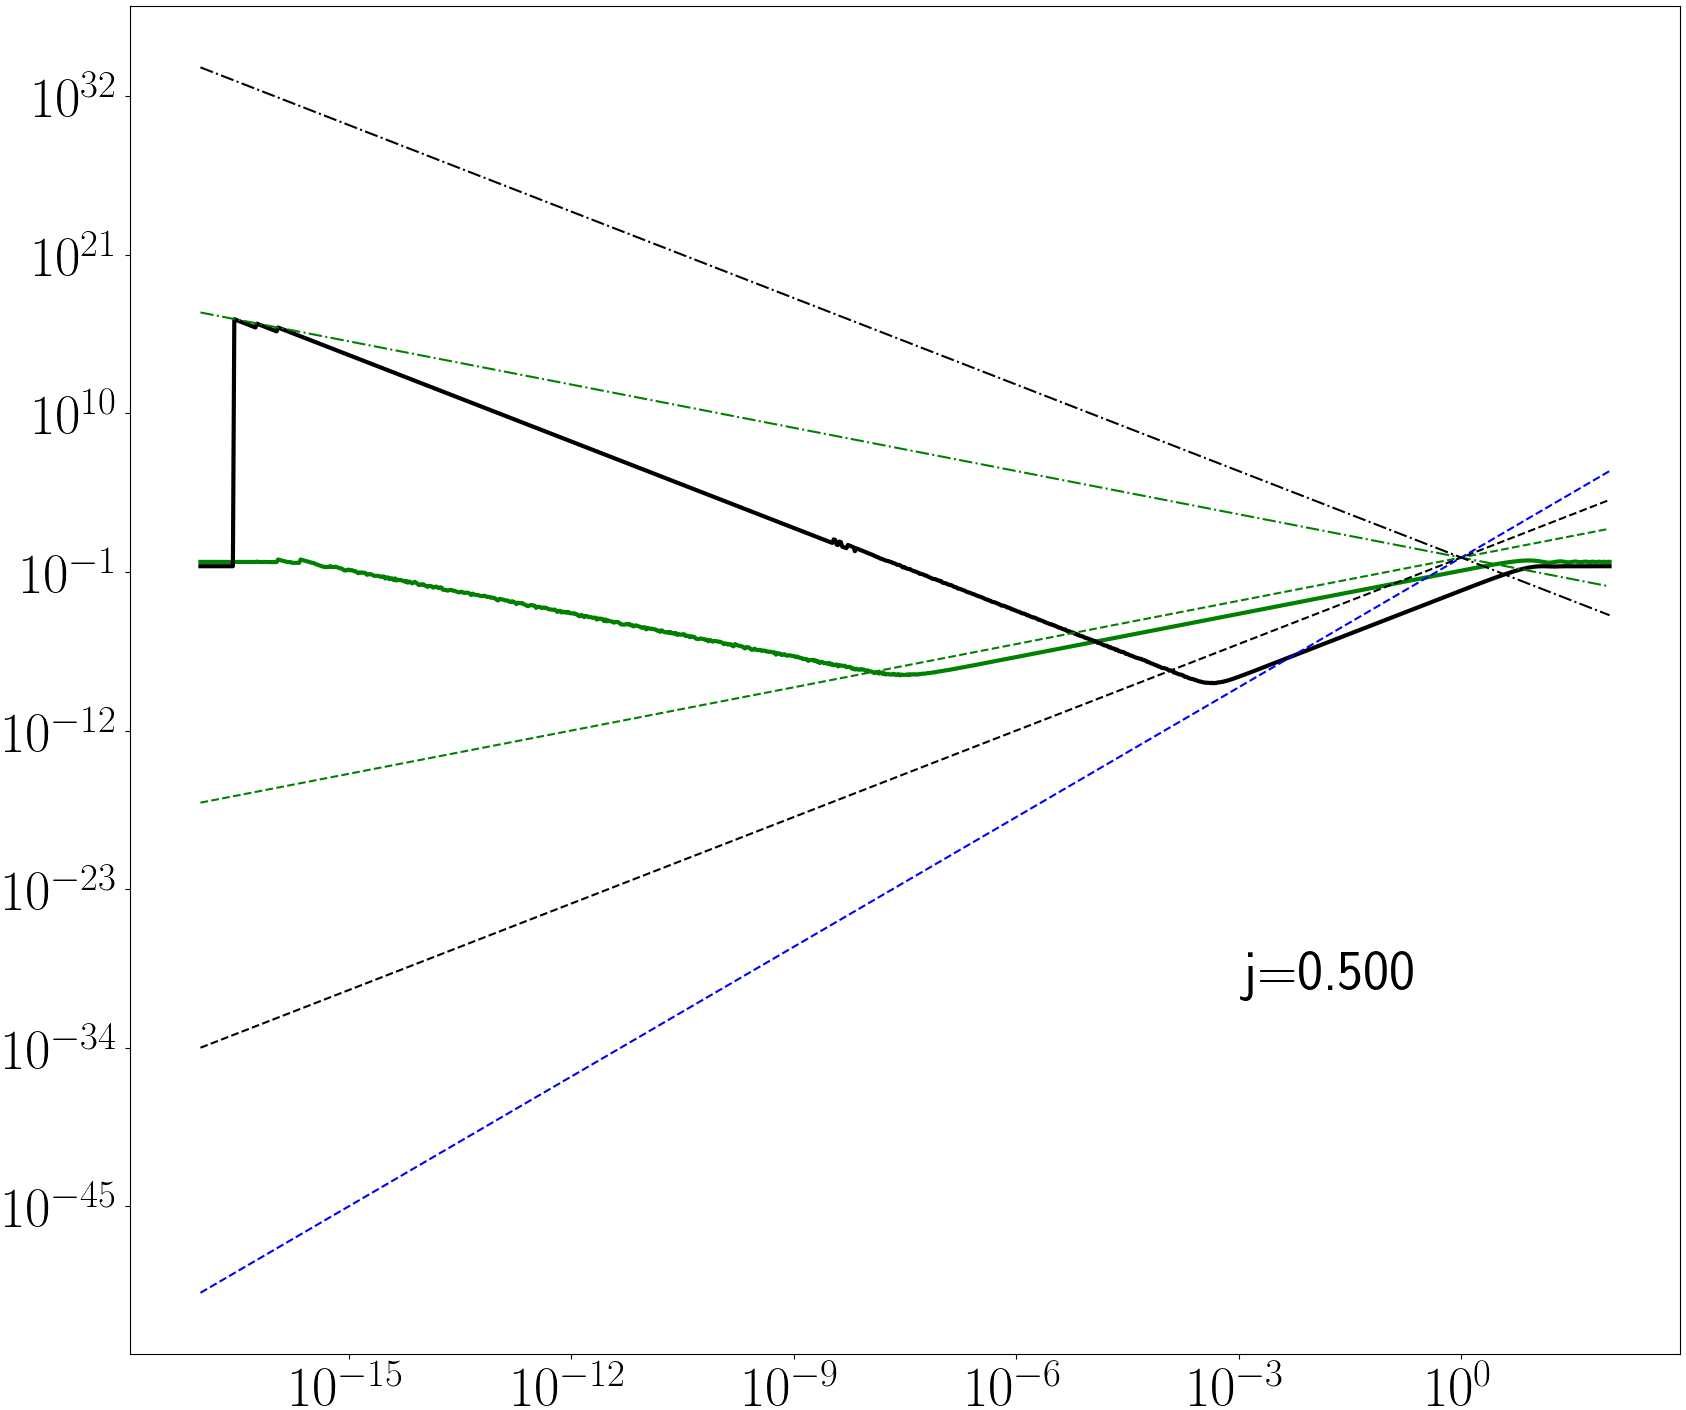
\includegraphics[width=.5\textwidth]{Bilder/errplot_0050.png}}
\subfigure[$j=4$]{\label{im:errplot_j_0400}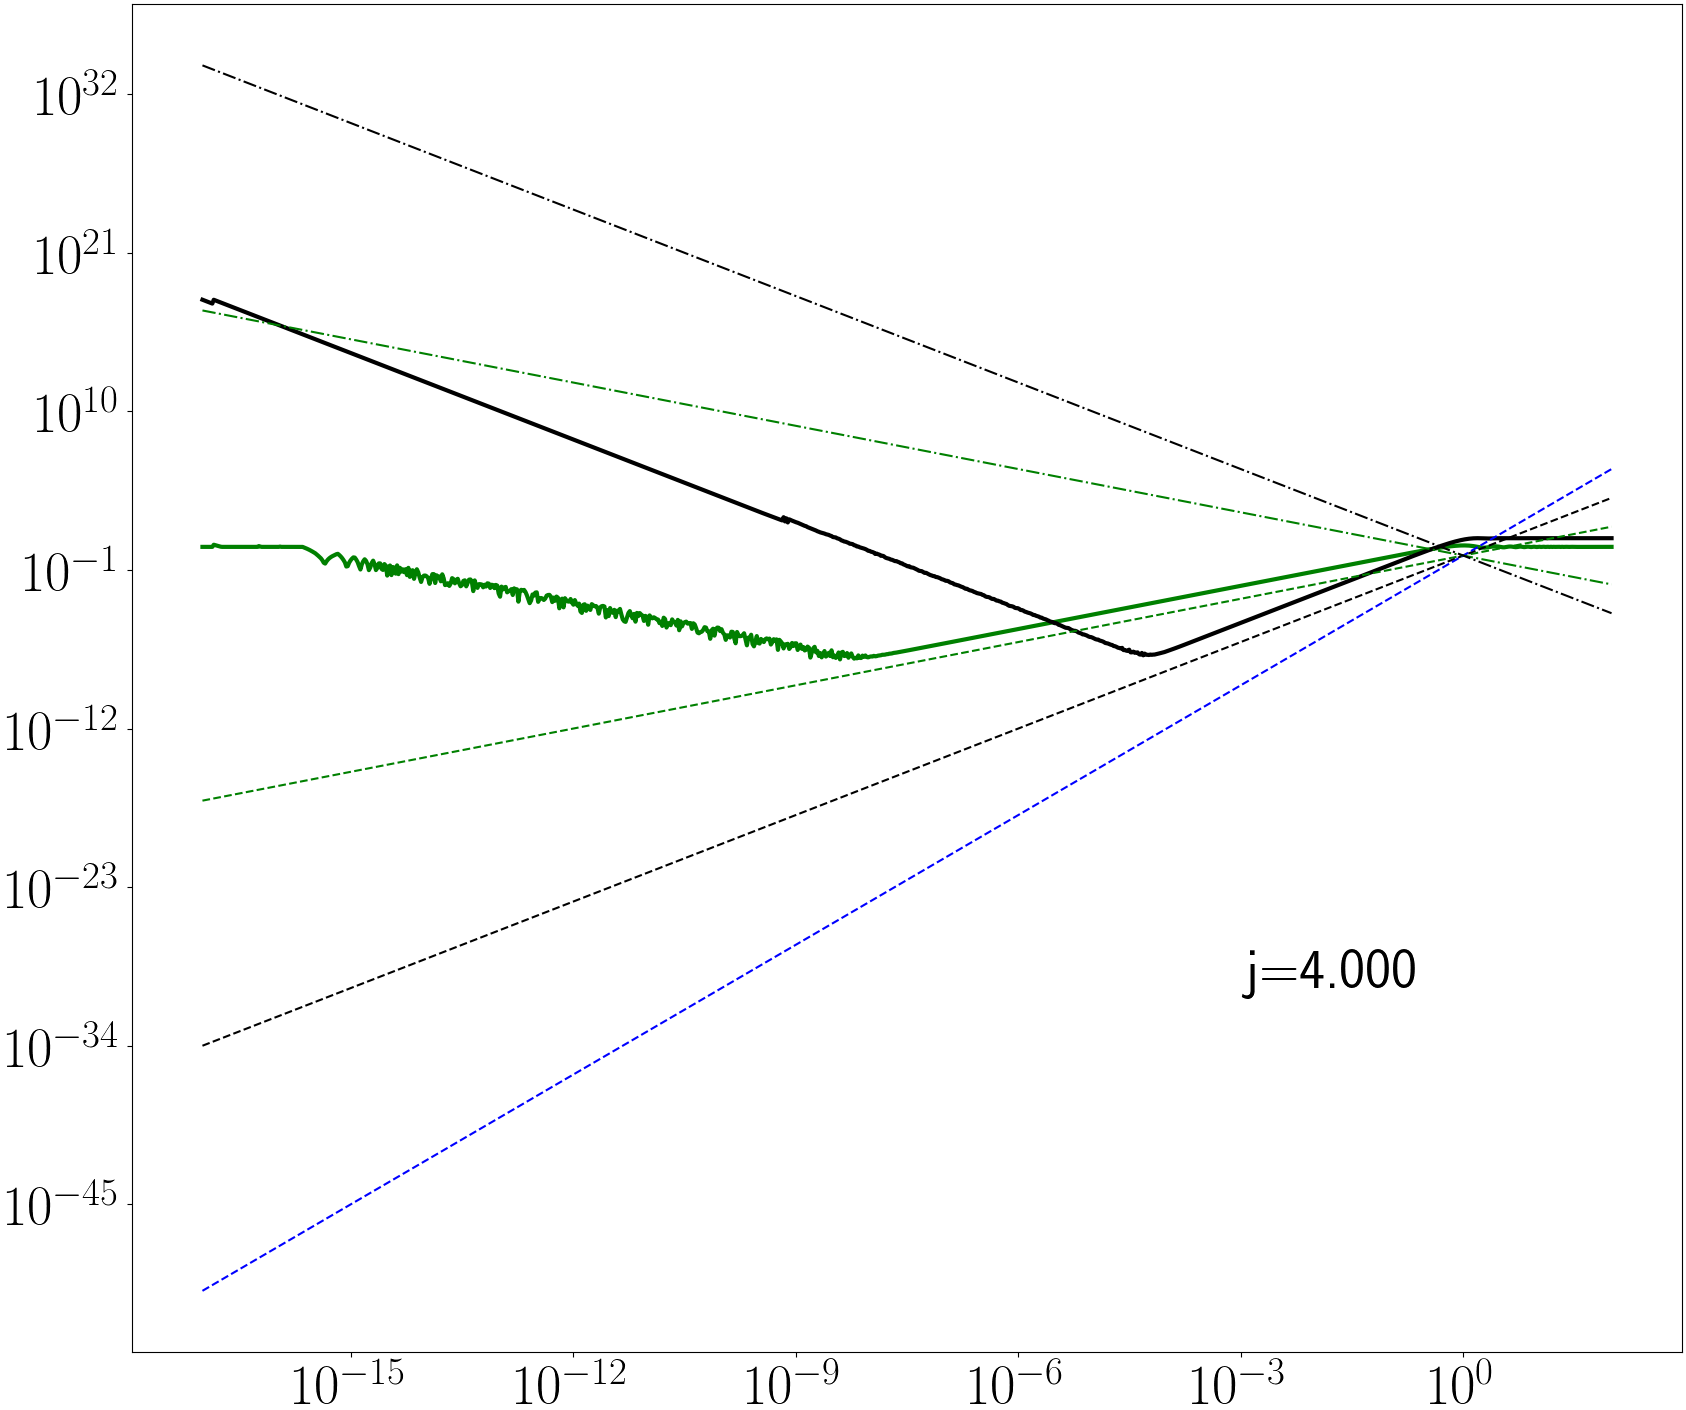
\includegraphics[width=.5\textwidth]{Bilder/errplot_0400.png}}
\subfigure[$j=50$]{\label{im:errplot_j_5000}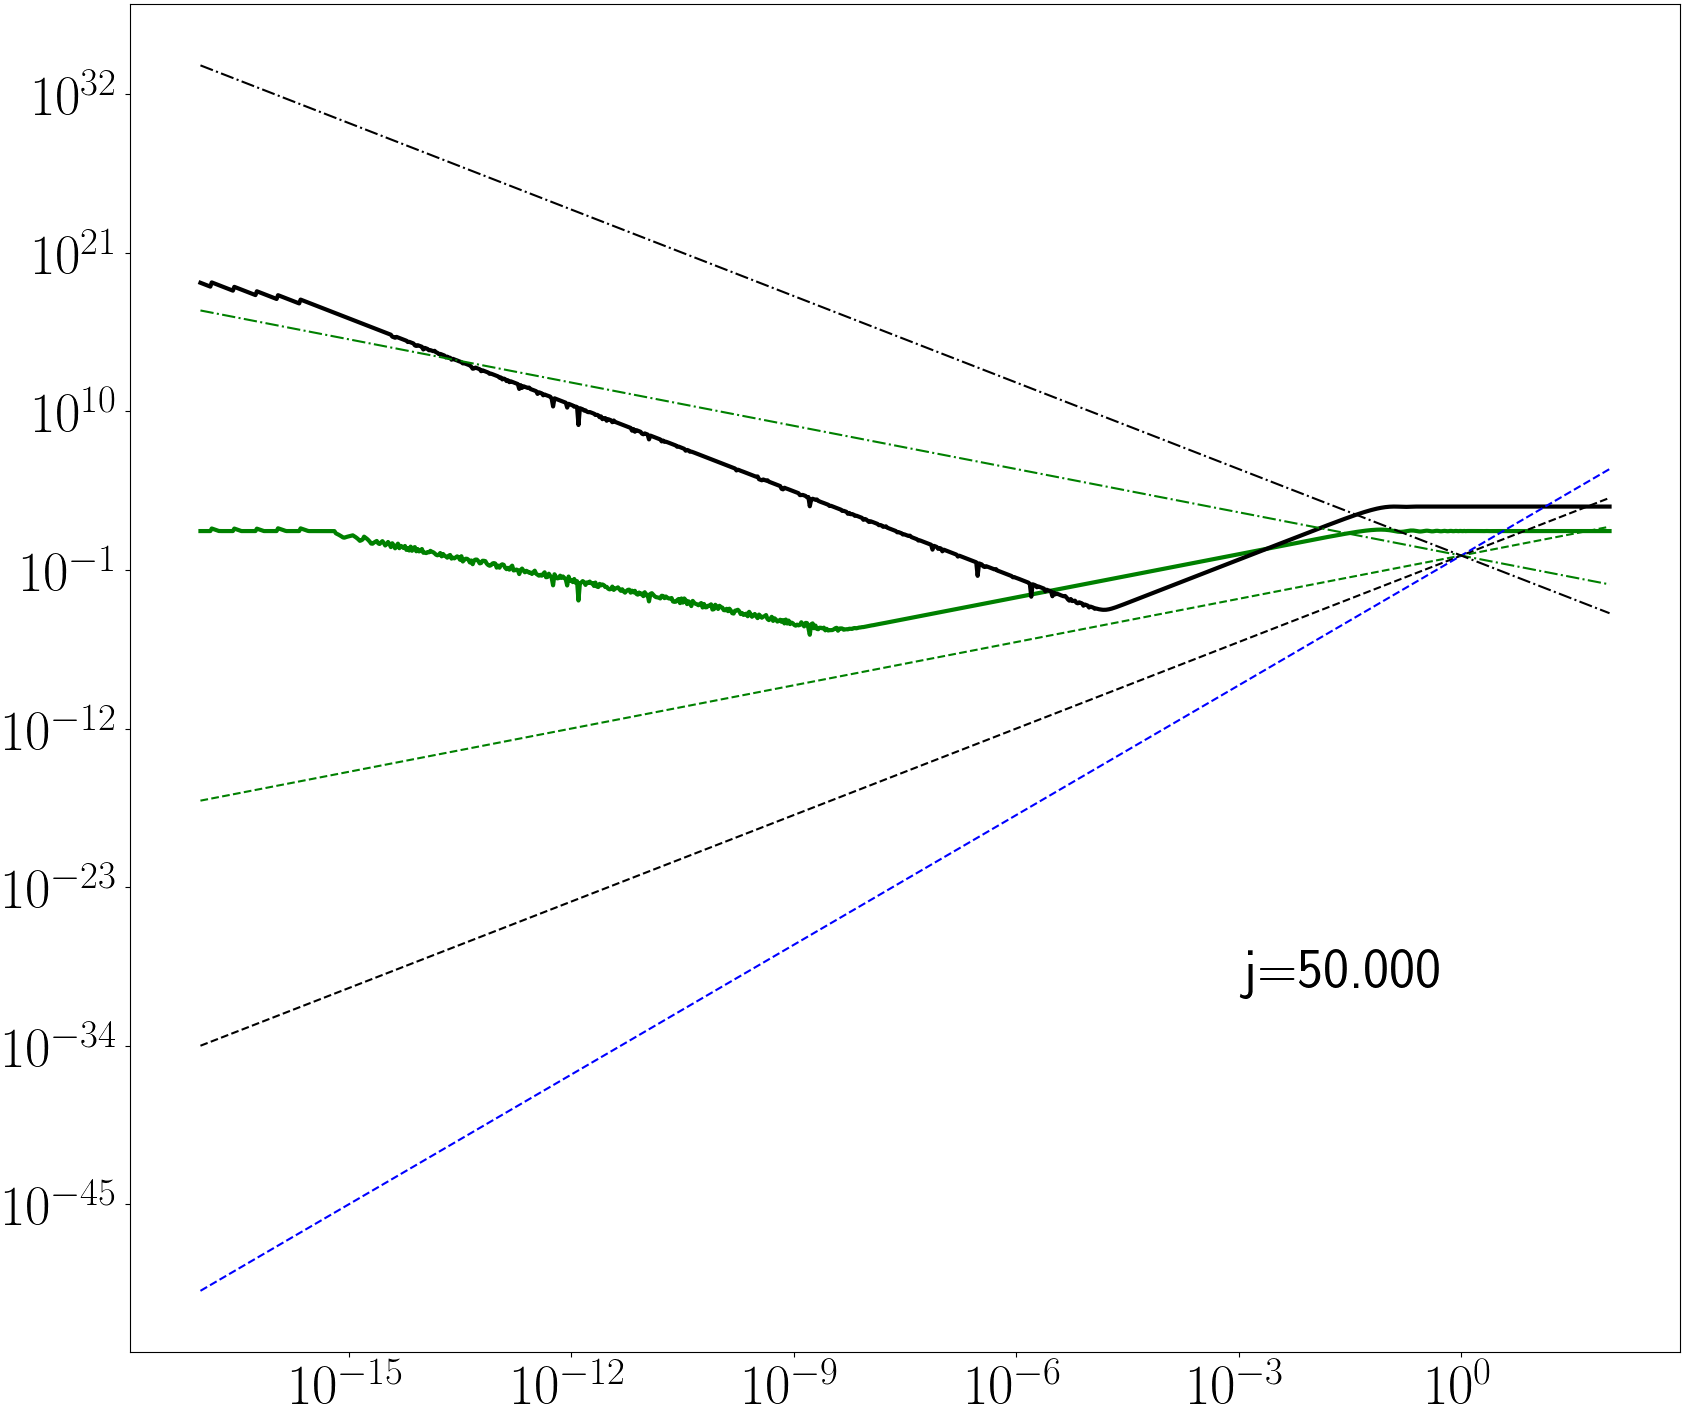
\includegraphics[width=.5\textwidth]{Bilder/errplot_5000.png}}
\subfigure[$j=100$]{\label{im:errplot_j_10000}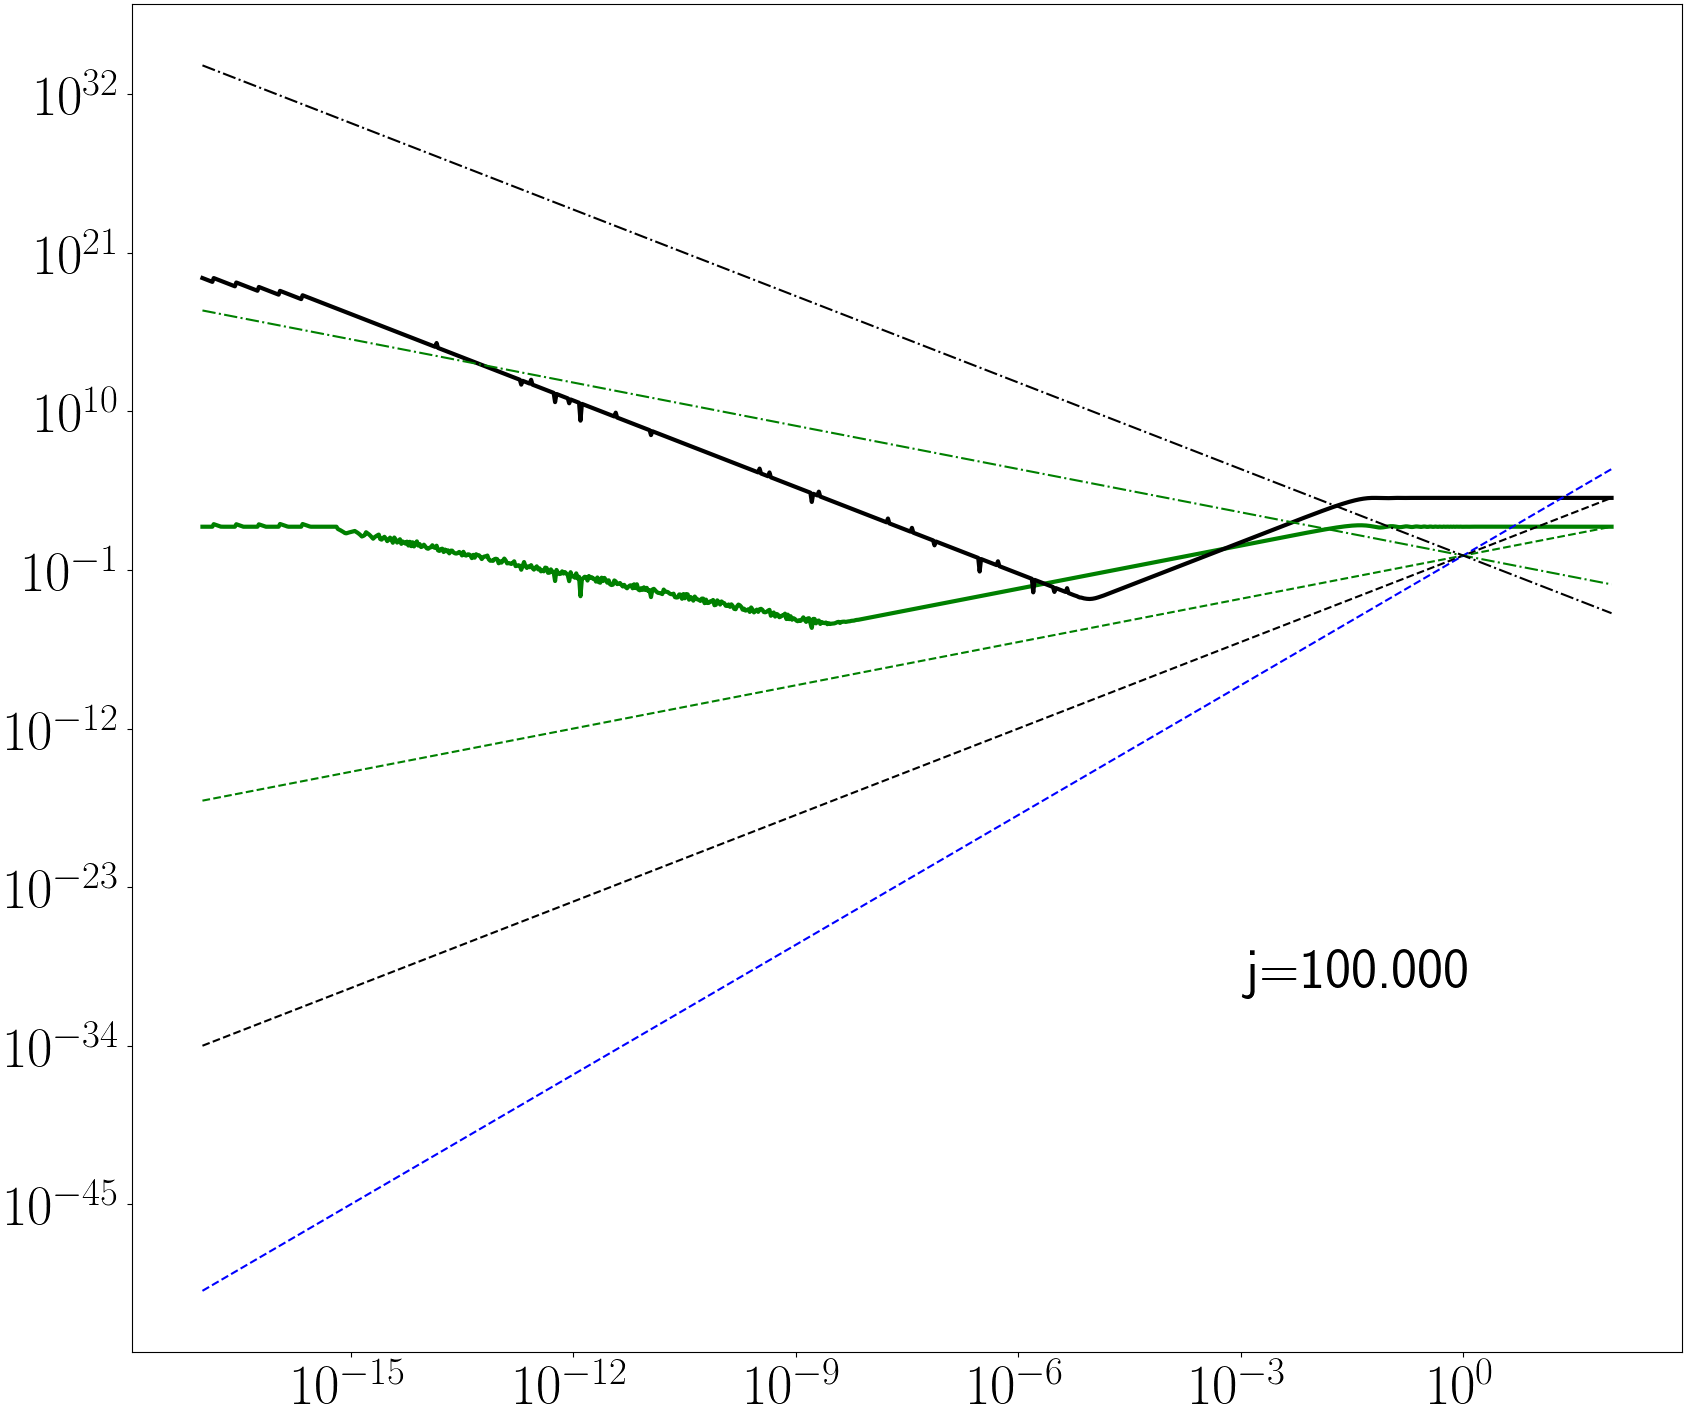
\includegraphics[width=.5\textwidth]{Bilder/errplot_10000.png}}
\caption{Fehlerverhalten der Approximation für verschiedene $j$}
\label{im:errplot_j}


\end{figure}



\section{Zusammenfassung}

Die Untersuchung des Maximalfehlers der Approximation der ersten beiden Ableitungen der Sinus-Funktion zeigte das erwartete Verhalten $e_h^{(k)}\sim h^{k}$ nur für etwa den Bereich $h\in\left[10^{-7},10^1\right]$ für die erste bzw.~$h\in\left[10^{-3},10^1\right]$ für die zweite Ableitung. Für kleinere $h$ ändert sich das Verhalten zu $e_h^{(k)}\sim h^{-k}$, moduliert mit einem Rauschen um ca. eine halbe Zehnerpotenz bishin zu $e_h^{(k)}=1$ für $h<10^{-17}$. Betrachtet man die Funktion $f_j(x)=\sin(jx)$, so ergeben sich ähnliche Verhalten der Approximationsfehler, allerdings verschieben sich die Bereiche der verschiedenen Konvergenzen mit Veränderung von $j$. So senkt sich zwar der Fehler für kleine $j$ für moderate  $h$-Werte, allerdings fängt auch der $\sim h^{-k}$-Bereich bereits bei höheren $h$ an. Es ist also ratsam, beim numerischen Differenzieren genau auf die Periodiziät der zu untersuchenden Funktion zu achten, um die Differenziationsschrittweite optimal zu wählen (diese liegt genau am Übergang des $\sim h^k$- und des $\sim h^{-k}$-Bereiches bei $h_{krit}^{(k)}$). Da die Ableitung einer periodischen Funktion wiederum periodisch ist, genügt es dabei, eine Periode zu untersuchen, was zusätzlich den numerischen Aufwand verringern kann, in dieser Aufgabenstellung aber nicht nötig war, sodass $f_j$ auch über Vielfaches seiner Periode hinweg untersucht werden konnte, ohne merkliche Performance-Verluste hinnehmen zu müssen.


%%% END OF DOCUMENT %%%%%%%%%%%%%%%%%%%%%%%%%%%%%%%%%%%%%%%%%%%%%%%%%%%%%%%%%%%
\end{document}
